\documentclass[conference]{IEEEtran}
\usepackage[main=portuguese,provide=*]{babel}
\usepackage{cite}
\usepackage{amsmath,amssymb,amsfonts}
\usepackage{graphicx}
\usepackage{textcomp}
\usepackage{xcolor}
\usepackage[hidelinks]{hyperref}
\usepackage{booktabs}

\begin{document}

\title{Multiplicação de Matrizes com MPI:\\
Versão Simples e Versão Blocada com Ladrilhos}

\author{
    \IEEEauthorblockN{
        \begin{tabular}{c}
            Gustavo Gabriel Ripka \\
            GRR20203935
        \end{tabular}
        \qquad \qquad
        \begin{tabular}{c}
            Arthur Barreto Godoi \\
            GRR20224377
        \end{tabular}
    }
    \vspace{0.2cm}
    \IEEEauthorblockA{
        \textit{Departamento de Informática} \\
        \textit{Universidade Federal do Paraná -- UFPR}\\
        Curitiba, Brasil
    }
}

\maketitle

\begin{abstract}
Este trabalho apresenta duas versões paralelas em MPI para a multiplicação
de matrizes de \texttt{double}, conforme a especificação do Trabalho 2 da
disciplina CI1316 (Programação Paralela, UFPR). A versão A é a formulação
simples: o nodo 0 inicializa A e B, distribui faixas de linhas de A com
\texttt{MPI\_Scatterv}, difunde B com \texttt{MPI\_Bcast} e reúne C com
\texttt{MPI\_Gatherv}; o kernel local é o laço triplo direto na ordem
$i \rightarrow k \rightarrow j$. A versão B mantém a mesma distribuição, mas
o kernel percorre a matriz em ladrilhos $w \times w$ com laços externos
$ii \rightarrow kk \rightarrow jj$, de modo que os blocos de A, B e C
permaneçam no cache, e a comunicação inicial usa operações coletivas não
bloqueantes (\texttt{MPI\_Ibcast} e \texttt{MPI\_Iscatterv}) sobrepostas.
Os experimentos foram executados no cluster Xeon da disciplina (Intel Xeon
E5410, 2,33~GHz, 2 soquetes de 4 núcleos, rede Gigabit Ethernet) via fila
Slurm, com um processo MPI por nodo exclusivo e média de 10 execuções para
matrizes $2304 \times 960$ por $960 \times 960$. A versão B foi sempre mais
rápida: 2,14$\times$ com 1 nodo e 1,61$\times$ com 4 nodos. A melhor vazão
absoluta foi de 4,21~GFLOPS (B, 4 nodos), contra 2,62~GFLOPS da versão A;
as acelerações sobre 1 nodo chegaram a 2,40$\times$ (B) e 3,19$\times$ (A),
limitadas pelo custo crescente das comunicações na rede Gigabit.
\end{abstract}

\section{Introdução}

O objetivo do trabalho é implementar, em um único programa C (\texttt{mmul.c},
executável \texttt{mmul}), duas versões paralelas em MPI da multiplicação de
matrizes quadradas de \texttt{double} e comparar o desempenho das duas no
cluster Xeon da disciplina. Dadas $A$ de ordem $Nla \times M$ e $B$ de ordem
$M \times Ncb$, calcula-se $C = A \cdot B$, de ordem $Nla \times Ncb$. A
inicialização é feita apenas no nodo 0, para evitar leitura de disco, e o
paralelismo usa exclusivamente MPI.

A versão A é a formulação ``normal, simples e direta'' do algoritmo; a versão
B é a versão blocada (\emph{tiling}), que explora a localidade de cache ao
processar a matriz em ladrilhos $w \times w$. O programa roda em dois modos:
medição (padrão), que reporta tempos e vazão, e verificador (\texttt{-v}), que
compara o resultado paralelo com uma execução sequencial exata, sem medir
tempo. O modo verificador foi executado no nodo de entrada \texttt{w00}, sem
Slurm, conforme recomendado no enunciado.

\section{Metodologia}

\subsection{Distribuição de dados e comunicação}

O nodo 0 aloca e inicializa as três matrizes e, a partir delas, os demais
processos recebem apenas o necessário para a computação:

\begin{itemize}
    \item \textbf{A:} distribuída por faixas contíguas de linhas com
    \texttt{MPI\_Scatterv}. Cada processo recebe $nl$ linhas de A, onde
    $nl = \lfloor Nla/n \rfloor$ mais uma linha extra para os primeiros
    $Nla \bmod n$ processos. Na versão A essa distribuição é genérica
    (não exige $Nla$ divisível por $n$).
    \item \textbf{B:} a matriz inteira é difundida para todos os processos
    com \texttt{MPI\_Bcast}, pois cada linha local de A precisa de todas as
    colunas de B.
    \item \textbf{C:} cada processo calcula a sua faixa local de C e o nodo 0
    reúne o resultado com \texttt{MPI\_Gatherv}.
\end{itemize}

Dessa forma, o tráfego de rede por processo é de $nl \cdot M$ elementos de A
e $M \cdot Ncb$ elementos de B na distribuição, e $nl \cdot Ncb$ elementos
de C na reunião.

\subsection{Versão A: kernel simples}

O kernel local percorre as $nl$ linhas da faixa e, para cada linha $i$,
acumula em $C[i][\cdot]$ a contribuição de cada $k$. A ordem adotada é
$i \rightarrow k \rightarrow j$, com o laço interno sobre $j$ contíguo em
memória. Não há blocagem: para cada linha de A a matriz B inteira é
percorrida uma vez.

\subsection{Versão B: kernel blocada com ladrilhos}

A versão B mantém exatamente a mesma distribuição de dados, mas muda o kernel
local. A faixa de $nl$ linhas é percorrida em blocos, com três laços externos
na ordem $ii \rightarrow kk \rightarrow jj$: $ii$ indexa blocos de linhas de
A e C, $kk$ indexa blocos de colunas de A (linhas de B) e $jj$ indexa blocos
de colunas de B e C. Para cada trio de blocos, um bloco $w \times w$ de B é
carregado no cache e reaproveitado pelas $w$ linhas do bloco de A, em vez de
ser relido para cada linha. Só o último bloco de linhas da faixa local pode
ser menor que $w$.

A escolha de $w$ busca manter três blocos simultaneamente no cache -- um de
A, um de B e um de C. Cada bloco de $192 \times 192$ \texttt{double} ocupa
$192^2 \cdot 8 = 294{,}9$~KiB; três blocos somam cerca de 885~KiB, folgados
no cache L2 de 12~MiB por soquete (3~MiB por núcleo), mas grandes o
suficiente para amortizar os acessos à memória. Além disso, $w = 192$ é
múltiplo de 8 e divide exatamente $M = Ncb = 960$ (5 blocos por linha de
blocos), como exigido pela simplificação da versão B. O programa também
valida essas restrições ($M$ e $Ncb$ múltiplos de 8 e de $w$, $w$ múltiplo de
8 e $Nla$ divisível por $n$).

\subsection{Comunicação não bloqueante e medição de tempos}

Na versão B a distribuição inicial usa \texttt{MPI\_Ibcast} para B e
\texttt{MPI\_Iscatterv} para A, disparadas juntas e concluídas com
\texttt{MPI\_Waitall}, de modo que o envio de B se sobrepõe à distribuição
de A. A medição usa a biblioteca \texttt{chrono.c} fornecida pelo professor:
um cronômetro mede o tempo total (da distribuição até a reunião de C) e
outro mede apenas a computação local. O tempo de comunicação é reportado
como a diferença entre os dois, como sugerido no enunciado. Como o tempo
total é ditado pelo processo mais lento, os tempos são reduzidos com
\texttt{MPI\_Reduce} (máximo) e reportados pelo nodo 0. A vazão é calculada
como $2 \cdot Nla \cdot M \cdot Ncb / t_{\text{total}}$, em GFLOPS. Para os
tamanhos medidos, o total de operações de ponto flutuante é de 4,247~GFLOP.

\subsection{Verificação da correção}

O modo verificador (\texttt{-v}) compara o resultado paralelo com uma versão
sequencial exata, antes de terminar o MPI e de desalocar as matrizes. A
função \texttt{verifica\_resultado} calcula $C_{aux} = A \cdot B$ de forma
sequencial, compara elemento por elemento com precisão exata (os valores são
inteiros pequenos, portanto a aritmética é exata em qualquer ordem de
somatório) e imprime o primeiro erro encontrado, retornando o número de
elementos divergentes. As matrizes são inicializadas no nodo 0 com
\texttt{srand(1)} e \texttt{gera\_matriz} (\texttt{rand()\%9 - 4}).

A verificação foi executada no nodo \texttt{w00} sem Slurm, com 4 processos,
tanto em tamanho reduzido ($512^3$, $w=64$) quanto no tamanho oficial
($2304 \times 960 \times 960$, $w=192$); em ambos os casos o resultado foi
considerado idêntico ao sequencial. A saída completa está em
\texttt{resultados/verificacao-w00.txt}.

\section{Processador}

A Tabela~\ref{tab:cpu} resume as características do processador dos nodos de
processamento do cluster. Trata-se de um Xeon Harpertown de 2007, com dois
soquetes de quatro núcleos, sem hyperthreading e sem AVX: cada nodo executa
no máximo 8 processos MPI sem \emph{oversubscribe}. O pico teórico de ponto
flutuante em precisão dupla (SSE, 2 multiplicações + 2 somas por ciclo por
núcleo) é da ordem de $2{,}33~\text{GHz} \times 8 \times 4 \approx
74{,}6$~GFLOPS por nodo. Os nodos se comunicam por Gigabit Ethernet. O texto
completo do \texttt{lscpu} e a figura do \texttt{lstopo} estão no apêndice.

\begin{table}[!t]
\caption{Características do processador (nodo do cluster Xeon).}
\label{tab:cpu}
\centering
\begin{tabular}{ll}
\toprule
Modelo          & Intel Xeon E5410 @ 2,33~GHz \\
Soquetes        & 2 \\
Núcleos/soquete & 4 (8 por nodo, sem SMT) \\
NUMA            & 1 nó \\
Cache L1d       & 32~KiB por núcleo (256~KiB total) \\
Cache L2        & 12~MiB por soquete (24~MiB total) \\
Conjuntos SSE   & até SSE4.1 (sem AVX) \\
Rede            & Gigabit Ethernet \\
\bottomrule
\end{tabular}
\end{table}

\section{Experimentos e Resultados}

\subsection{Metodologia experimental}

As medições seguiram o enunciado: matrizes $A = 2304 \times 960$ e
$B = 960 \times 960$ (logo $C = 2304 \times 960$), 1 a 4 nodos, modo
exclusivo (\texttt{sbatch --exclusive -N n}), um processo MPI por nodo
(\texttt{mpirun --map-by ppr:1:node}) e 10 execuções por configuração,
reportando-se a média. Cada processo imprime o seu rank e o nome do host,
o que confirmou a alocação de um processo por nodo (por exemplo, ranks 0 e 1
em \texttt{wz10} e \texttt{wz11}). Os jobs oficiais foram submetidos à fila
\texttt{debug} (limite de 5 minutos) e as saídas brutas, com os
identificadores dos jobs (19338 a 19345), estão em \texttt{resultados/}.

\begin{table}[!t]
\caption{Versão A (simples): médias de 10 execuções.}
\label{tab:expA}
\centering
\begin{tabular}{rrrrrr}
\toprule
nodos & $t$ total (s) & $t$ comp. (s) & $t$ com. (s) & GFLOPS & acel. \\
\midrule
1 & 5,1723 & 5,1255 & 0,0467 & 0,821 & 1,000 \\
2 & 2,8945 & 2,6479 & 0,2466 & 1,468 & 1,787 \\
3 & 2,0232 & 1,7602 & 0,2630 & 2,099 & 2,556 \\
4 & 1,6231 & 1,3223 & 0,3008 & 2,617 & 3,187 \\
\bottomrule
\end{tabular}
\end{table}

\begin{table}[!t]
\caption{Versão B (blocada, $w = 192$): médias de 10 execuções.}
\label{tab:expB}
\centering
\begin{tabular}{rrrrrr}
\toprule
nodos & $t$ total (s) & $t$ comp. (s) & $t$ com. (s) & GFLOPS & acel. \\
\midrule
1 & 2,4188 & 2,3727 & 0,0461 & 1,756 & 1,000 \\
2 & 1,4068 & 1,1732 & 0,2336 & 3,019 & 1,719 \\
3 & 1,1371 & 0,7981 & 0,3391 & 3,735 & 2,127 \\
4 & 1,0086 & 0,5977 & 0,4109 & 4,211 & 2,398 \\
\bottomrule
\end{tabular}
\end{table}

\begin{table}[!t]
\caption{Comparação das versões: aceleração de B em relação a A.}
\label{tab:comp}
\centering
\begin{tabular}{rrrrr}
\toprule
nodos & $t$ A (s) & $t$ B (s) & aceleração B/A & GFLOPS B \\
\midrule
1 & 5,1723 & 2,4188 & 2,138 & 1,756 \\
2 & 2,8945 & 1,4068 & 2,058 & 3,019 \\
3 & 2,0232 & 1,1371 & 1,779 & 3,735 \\
4 & 1,6231 & 1,0086 & 1,609 & 4,211 \\
\bottomrule
\end{tabular}
\end{table}

\begin{figure}[!t]
\centering
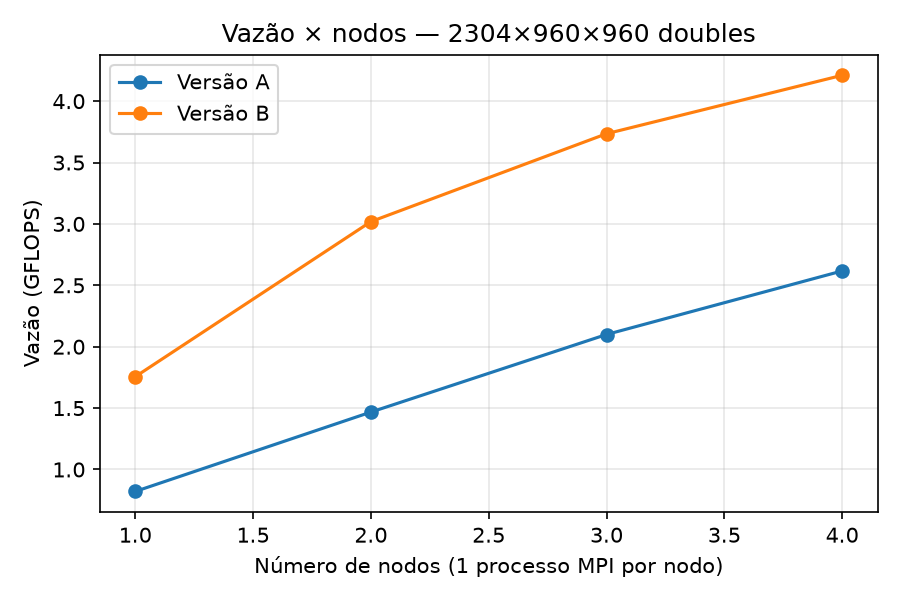
\includegraphics[width=\columnwidth]{figuras/grafico-vazao.png}
\caption{Vazão (GFLOPS) em função do número de nodos, versões A e B.}
\label{fig:vazao}
\end{figure}

\begin{figure}[!t]
\centering
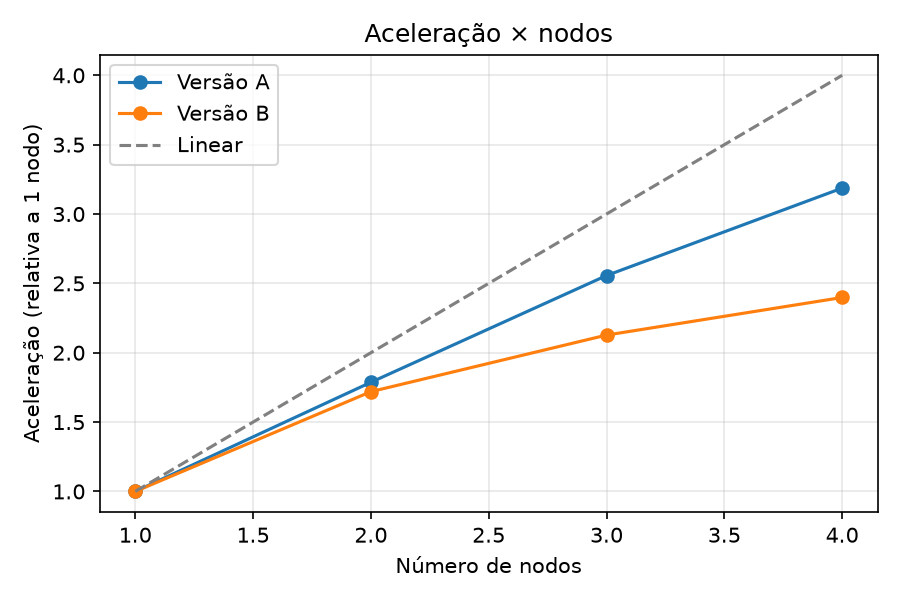
\includegraphics[width=\columnwidth]{figuras/grafico-aceleracao.png}
\caption{Aceleração relativa a 1 nodo, versões A e B, com a reta linear.}
\label{fig:acel}
\end{figure}

\begin{figure}[!t]
\centering
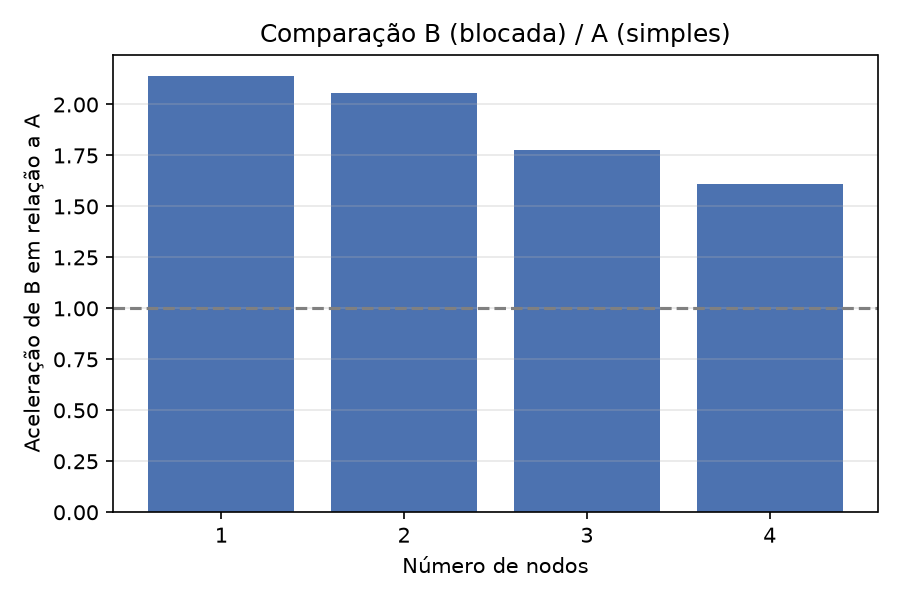
\includegraphics[width=\columnwidth]{figuras/grafico-b-vs-a.png}
\caption{Aceleração da versão B em relação à versão A para cada número de
nodos.}
\label{fig:bva}
\end{figure}

\begin{figure}[!t]
\centering
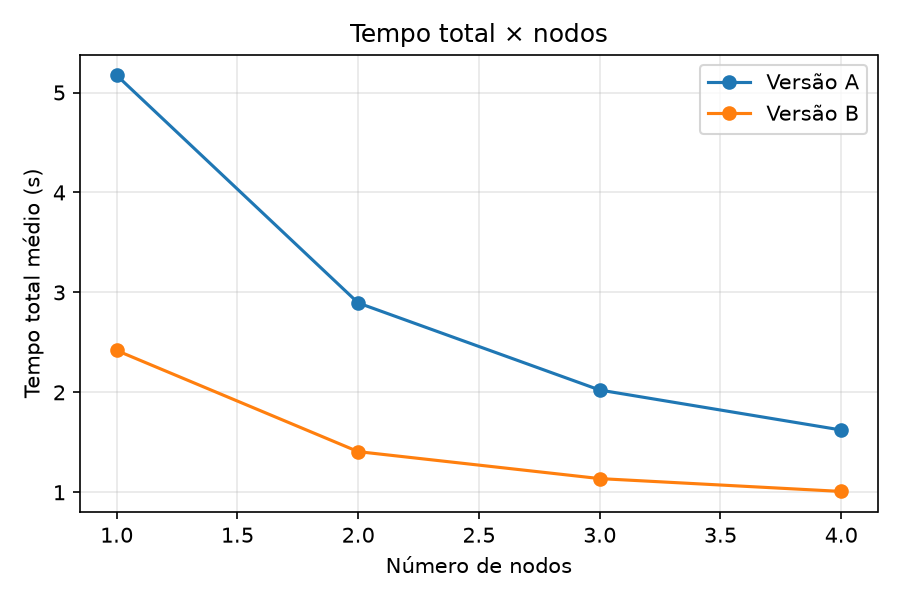
\includegraphics[width=\columnwidth]{figuras/grafico-tempo.png}
\caption{Tempo total médio em função do número de nodos.}
\label{fig:tempo}
\end{figure}

\section{Discussão}

\paragraph{Versão B contra versão A}
A versão B foi sistematicamente mais rápida, mesmo com o mesmo número de
processos e a mesma distribuição de dados: 2,14$\times$ com 1 nodo,
2,06$\times$ com 2, 1,78$\times$ com 3 e 1,61$\times$ com 4 (Tabela~\ref{tab:comp}
e Fig.~\ref{fig:bva}). A diferença vem exclusivamente do kernel local. Na
versão A, para cada linha de A a matriz B inteira é relida da memória; como
B tem $960 \cdot 960 \cdot 8 \approx 7{,}4$~MiB, o volume de leitura por
nodo é $nl \times 7{,}4$~MiB, muito acima do cache L2, o que torna o kernel
limitado pela largura de banda de memória. Na versão B, cada bloco de B
permanece no cache enquanto é usado pelas $w = 192$ linhas do bloco de A,
reduzindo o tráfego efetivo à memória por um fator próximo de $w$.

Observa-se também que a vantagem relativa de B diminui com o número de
nodos (2,14$\times$ com 1 nodo contra 1,61$\times$ com 4). Isso é esperado:
com mais nodos o tempo de computação por nodo cai, mas o tempo de
comunicação cresce (a matriz A a distribuir por nodo diminui, porém B
continua sendo difundida inteira e C é reunida no nodo 0), então a fração
de tempo gasta em comunicação -- igual nas duas versões -- passa a pesar
mais no tempo total.

\paragraph{Escalabilidade}
A computação local escala quase linearmente nas duas versões: na versão B,
o tempo de computação cai de 2,3727~s (1 nodo) para 1,1732~s (2 nodos),
0,7981~s (3) e 0,5977~s (4), isto é, eficiências de 101\%, 99\% e 99\% em
relação ao caso ideal. Na versão A, o mesmo ocorre (5,1255~s para 2,6479;
1,7602; 1,3223~s). A aceleração total, porém, fica abaixo do linear
(Fig.~\ref{fig:acel}): 3,19$\times$ com 4 nodos na versão A e 2,40$\times$
na versão B. A razão é o custo de comunicação na rede Gigabit: na versão B
com 4 nodos, 0,4109~s dos 1,0086~s totais (cerca de 41\%) são comunicação.
Como B computa muito mais rápido, a comunicação relativa cresce e limita a
aceleração; na versão A, que é mais lenta, a comunicação é proporcionalmente
menor (0,3008~s em 1,6231~s, cerca de 19\%), o que explica a aceleração
total maior apesar do kernel pior.

\paragraph{Absolutos}
As vazões absolutas (0,82 a 4,21~GFLOPS) representam apenas 1,1\% a 5,6\% do
pico teórico do nodo (cerca de 74,6~GFLOPS em precisão dupla). Isso se
explica por três fatores: o hardware é de 2007, sem AVX e com FSB, o kernel
não é vetorizado manualmente nem usa \emph{blocking} de registradores, e as
matrizes são grandes em relação ao cache, de modo que o desempenho é
dominado pela hierarquia de memória. A comparação A contra B mostra que a
otimização de cache é o fator mais importante disponível neste hardware: ela
sozinha vale mais que o dobro da vazão.

\section{Conclusão}

As duas versões paralelas foram implementadas em um único programa
\texttt{mmul.c}, com distribuição por \texttt{Scatterv}/\texttt{Bcast} e
reunião por \texttt{Gatherv}, medição separada de computação e comunicação
com a biblioteca \texttt{chrono}, e modo verificador exato. A versão blocada
com ladrilhos de $192 \times 192$ foi consistentemente superior à versão
simples, com ganho de 1,61$\times$ a 2,14$\times$, confirmando que a
localidade de cache é determinante na multiplicação de matrizes. As
acelerações com 4 nodos (3,19$\times$ na versão A e 2,40$\times$ na versão
B) ficaram limitadas pela rede Gigabit, cujo custo de comunicação chega a
41\% do tempo total na versão blocada. Como trabalho futuro, o uso de
comunicação não bloqueante também na reunião de C, de \emph{pipelining} por
blocos de linhas e de vetorização explícita permitiria atacar exatamente
esses dois limitantes.

\section*{Repositório}

O código-fonte, os scripts de experimento, as saídas brutas dos jobs e a
planilha estão disponíveis em
\url{https://github.com/gg-gustavo/mmul-mpi-blocado}.

\section*{Apêndice --- \texttt{lscpu} e \texttt{lstopo}}

{\footnotesize
\begin{verbatim}
Architecture:          x86_64
CPU(s):                8
Thread(s) per core:    1
Core(s) per socket:    4
Socket(s):             2
Model name:            Intel Xeon E5410 @ 2.33GHz
CPU MHz:               2327.471
L1d cache:             256 KiB
L1i cache:             256 KiB
L2 cache:              24 MiB
NUMA node0 CPU(s):     0-7
\end{verbatim}
}

\begin{figure}[!h]
\centering
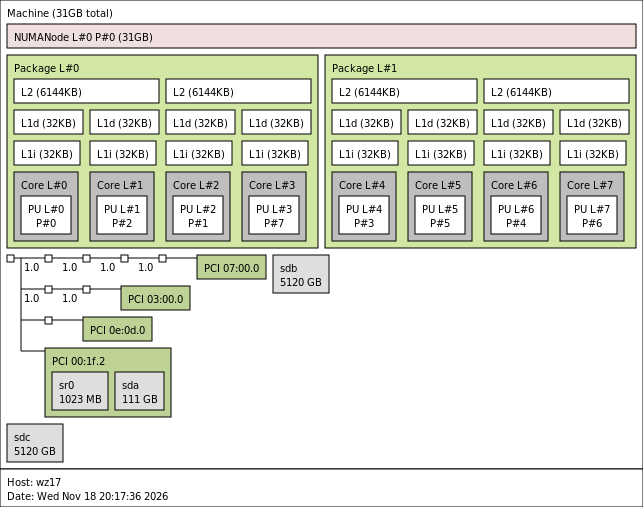
\includegraphics[width=\columnwidth]{lstopo-nodo.png}
\caption{Topologia do nodo do cluster (\texttt{lstopo}).}
\label{fig:lstopo}
\end{figure}

\end{document}
